\chapter{}
Agora mais tranquila, pude concentrar-me na superação do meu outro receio: o da formação escolar dos meus filhos.


A Fundação Bradesco, sob muitos aspectos, era uma escola maravilhosa, sobretudo quanto às instalações físicas.
As crianças jamais conheceriam escola tão bonita.
Localizada à beira do Rio Araguaia, era a unidade pioneira da rede, instalada numa antiga fazenda de propriedade de Amador de Aguiar, o fundador do banco, e onde ainda morava uma velha tia dele.
Por isso, a escola de Conceição, dizia-se, era a menina dos olhos do austero banqueiro.
A diretora, uma negra retinta, D.Auzelina Rosa, era firme e dedicada.
O problema era o corpo docente.
Aqui e ali, havia surpresas.
Uma ótima alfabetizadora, uma boa professora de Ciências, formada em São Paulo, uma excelente professora de quarta série que Tomaz adorava e um professor de Educação Física muito criativo, que gostava de dar aulas numa ilhota que brotara do rio, diante da escola.
Mas a grande maioria era gente formada no próprio estabelecimento e que mal acompanhava as orientações vindas da Cidade de Deus, a matriz de São Paulo.
Os que haviam completado o colegial lecionavam de quinta a oitava séries; os que tinham completado o segundo grau lecionavam de primeira a quarta séries.
À tarde, depois que almoçávamos, eu tinha que rever com Tomaz, Marcelo e, nos anos seguintes, com Fernando e Paula, todas as aulas, utilizando o material que havia trazido de Araraquara e aproveitando para corrigir as falhas e os erros, sobretudo os de português, cometidos pelos heróicos professores.

Havia, por outro lado, aspectos muito positivos na educação ministrada pela Fundação.
Amador Aguiar tinha a virtude de ser intransigente na exigência de que nas suas escolas vigorasse o seu credo pessoal: o culto ao trabalho, à disciplina e à organização.
Os alunos recebiam todo o necessário para estudar na escola.
Sapatinhos de lona, meias, mochila, calções, camisetas e uniforme de ginástica.
Duas vezes ao ano.
E todo o material escolar.
Não me foi permitido comprar uma borracha sequer para os meus filhos.

\textit{``-- Para que não haja o risco de se estabelecer diferenças entre os alunos.''}, explicou polidamente a diretora.
Ao final do ano, os livros deveriam ser devolvidos em perfeita ordem para serem reutilizados pelos alunos seguintes.
Todas as crianças eram diariamente examinadas no portão de entrada.
Unhas, cabelos, limpeza das meias e camisetas brancas, tudo passava por avaliação rigorosa.
Ao menor sinal de desmazelo, o aluno era inapelavelmente devolvido à casa.
À exceção dos meus filhos e de alguns outros filhos de funcionários lotados na cidade, a imensa maioria daqueles meninos e meninas eram filhos de ribeirinhos, pobres como Jó, moradores de casebres de pau-a-pique, cujas mães lavavam as roupas no rio.
Contudo, era raro que algum fosse reprovado no exame, exceto, às vezes, pela presença de piolhos.
Nesse caso, eram encaminhados para a enfermaria e recebiam imediatamente o remédio e as instruções para eliminá-los.

As aulas dedicadas ao aprendizado de trabalhos manuais, ao contrário do que costuma acontecer nas escolas desse país, eram levadas a sério.
Tomaz se orgulha de ter feito, na marcenaria, alguns dos banquinhos que o Bradesco distribuiu de brinde aos clientes no Natal de 82 ou 83.
Meninos e meninas tinham que aprender também a cultivar hortaliças, frutas e legumes que depois eram consumidos na refeição servida aos alunos diariamente, na hora do recreio.

E havia o aprendizado de Matemática, levado com absoluto rigor.
A primeira aula dos meninos consistia em aprender a construir o seu próprio \textit{soroban}, um ábaco em versão japonesa, destinado a desenvolver a capacidade de cálculo mental e fantástico para facilitar o aprendizado dos numerais e da sua ordenação.
Era outra exigência inarredável do velho banqueiro.

A limpeza da escola e o cuidado com os jardins era o que mais me encantava.
Contaram-me que Amador Aguiar tinha o hábito de aparecer sem avisar.
Deixava o carro na cidade e vinha a pé pela estrada, entrando na escola despercebido.
E um papel esquecido no chão que ele se abaixasse para catar, uma samambaia murcha por falta de água ou um galho arrancado por vandalismo dos alunos, era motivo para que ele descompusesse a diretora nos termos mais rudes ou até a despedisse, como chegou a acontecer alguns anos antes da nossa chegada.
Dessa maneira, toda a escola brilhava, as plantas eram sagradas e os banheiros eram vigiados e lavados de cima a baixo após cada intervalo.
  
Para finalizar, todas as crianças eram submetidas semestralmente a exame médico e dentário e recebiam tratamento gratuito para os problemas detectados.

Não importa quantos pecados Amador Aguiar possa ter cometido nesse mundo e Deus sabe que os banqueiros desse país têm muitas contas a acertar lá do outro lado, mas a obra que ele desenvolveu por intermédio dessa Fundação, tenho certeza, deve tê-lo redimido de quase todos eles, se não de todos.
Bendito seja.

Quando Fernando frequentava já o primeiro ano na Fundação Bradesco, numa reunião de pais aí pelo mês de junho, Auzelina e a professora me chamaram para perguntar como acontecia de Fernando já estar alfabetizado naquela altura, enquanto o resto da classe mal reconhecia as vogais.

\textit{``-- Fernando foi o único que conseguiu?''}, perguntei.

\textit{``-- Fernando e aquele garotinho ali.''}, respondeu a professora, apontando para um negrinho miúdo, acompanhado da mãe, miúda também e de aparência muito humilde.

\textit{``-- Bom''}, eu disse, \textit{``terei o maior prazer em por à disposição de vocês os materiais que utilizo com as crianças em casa, mas, dadas as condições da maioria das crianças, não seria interessante também saber como é que aquele menininho deu conta de aprender?''} 

Fomos conversar com a mãe.

\textit{``-- Conte-nos, o que a senhora faz para que seu menino se saia tão bem na escola?''}

Com um sorriso tímido, ela entregou o segredo:

\textit{``-- Eu sou analfabeta e meu maior sonho, meu menino sabe, era que ele aprendesse a ler e escrever.
Então, à noite, enquanto ele faz a tarefa, eu escolho o feijão sentada ali perto e vou pedindo para ele ler tudo para mim, o que está nos livros e todos aqueles sinaizinhos que ele vai fazendo no caderno.
Acho bonito demais!'' }

Essa incrível receita de dar importância a um filho e fazê-lo ter orgulho de estudar, eu a repassei, como coordenadora pedagógica, a todos os pais que me perguntaram o que fazer com os preguiçosos que tinham em casa.

Aos poucos, fomos entrando na rotina da cidadezinha.
A escola e o rio balizavam a minha vida e a dos meninos.
Não havia cinema, nem \textit{shoppings} e a televisão só funcionava enquanto o gerador não era desligado e, na verdade, não fazia falta.
À noite líamos ou escrevíamos cartas para os parentes, cheias de desenhos de bichos, plantas, voadeiras...As crianças pareciam felizes.
Alheias às minhas preocupações, desfrutavam uma infância de sonhos há muito perdida para os meninos de cidade grande: nadavam no rio, subiam em árvores, andavam de canoa, pescavam.
Roupa, só quando iam para a escola.
Na maior parte do tempo não se distinguiam dos outros pequenos do lugar, andando só de calção e chinelinho de borracha.
O clima, uniformemente quente o ano inteiro, não exigia mais.
Quando escurecia, o vento da mata tornava o ar bem mais fresco e dormia-se bem.
Nos fins de semana, Paulo nos levava para uma das fazendas e aí era uma festa.
Ou então, íamos comer num dos dois restaurantes do lugar, o Taboquinha ou o Fauze, instalado num barco encalhado à margem do rio e que oferecia cardápio fixo: pacu frito, farinha e salada.
Definida a quantidade pelo freguês, uns moleques que esperavam por perto mergulhavam na água e logo voltavam à superfície para entregar os peixes vivíssimos à cozinheira que os aguardava na janela da cabine.
Ali mesmo os bichinhos eram estripados e limpos e menos de quinze minutos depois, o pedido chegava à mesa, quente, crocante e cheiroso.
Meus filhos vibravam.

Só o Vicente permanecia recalcitrante.
De pé, agarrado à alça do painel da Belina, me acompanhava por todo lado, carinha amarrada.
Um dia, voltando da casa do ``Copila'', um piloto conhecido do Paulo, cujos filhos se tornaram amigos dos nossos, destampou de repente:

\textit{``-- Quando crescer,  vou virar piloto e comprar um avião.''}

\textit{``-- É mesmo, filho? Para voar por cima da floresta, como o Copila?''}, indaguei.

E ele:
\textit{``-- Não.
Para sair daqui voando e voltar para Araraquara.''}

Em julho, acontecia o auge da vazante do Araguaia.
O fundo do rio aflorava em ilhas, ou coroas, como eram chamadas.
Já em junho a população entrava em grandes preparativos, na expectativa desse acontecimento.
Peões eram contratados para construir grandes ranchos nessas coroas e apenas começavam as férias escolares, as famílias se mudavam para lá com armas e bagagens e de lá só retornavam quando as águas voltavam a subir.
Muitos, só quando o rio lhes chegava aos joelhos.
O Taboquinha, por exemplo, o melhor restaurante da cidade, só abria nesse período porque na temporada da cheia ele permanecia submerso.
Famosos pelo maravilhoso tucunaré na brasa que serviam, os donos do Taboquinha mantinham as portas abertas até que, com a chegada das chuvas nas cabeceiras, o rio crescia e ameaçava cobrir o tampo das mesas.
E os clientes não se importavam de deixar os sapatos no alto da barranca do rio e, de roupas arrepanhadas, almoçar chapinhando na água, até o dia em que o restaurante fechava suas portas para reabri-las no ano seguinte.
Tampouco os garçons ou os cozinheiros se importavam em trabalhar de calças sungadas, com água acima das canelas.

As praias do Araguaia eram a maior alegria das crianças e embora eu tenha resistido à ideia de acampar nelas, não deixamos de participar da farra de julho, fazendo churrasco com os amigos e nadando nas águas quentes do rio, sempre atentos para não acabar fisgados pelas traiçoeiras arraias.

\begin{figure}
\centering
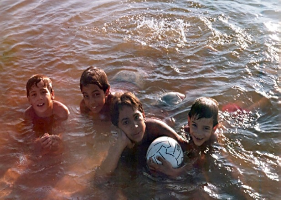
\includegraphics[width=0.7\linewidth]{31/praia- araguaia-1.png}
\end{figure}

\begin{figure}\ContinuedFloat
\centering
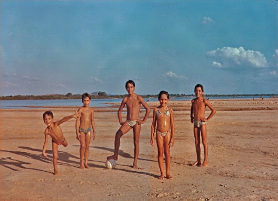
\includegraphics[width=0.7\linewidth]{31/praia- araguaia-2.png}
\caption{As praias e as águas mornas do Araguaia.}
\end{figure}

\begin{figure}
\centering
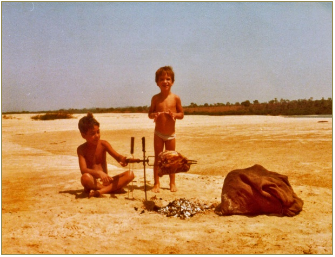
\includegraphics[width=0.7\linewidth]{31/churras.png}
\caption{Churrasco na coroa do rio.}
\end{figure}

\begin{figure}
\centering
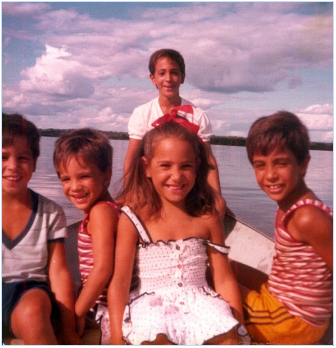
\includegraphics[width=0.7\linewidth]{31/voadeira.png}
\caption{Navegando na voadeira.}
\end{figure}

Nossos maiores amigos lá, além de Zezão e a mulher, Narcisa, eram Zé Antonio e Fátima, esta última, a meiga dentista das crianças.
Na esquina de casa morava Nilza, casada com o dono do posto de gasolina, uma figura engraçadíssima, brasiliense, fala enjoada de madame, mas, na realidade, o oposto disso, uma negociante muito esperta.
Foi a primeira pessoa com que travei conhecimento, pois mal tínhamos nos mudado, apareceu no meu portão para convidar-nos para o aniversário do marido.
Aceitamos prontamente o convite e, na festa, tive um pequeno vislumbre dos costumes locais.

Como acontece com certa frequência nas cidades do interior, logo à chegada, mulheres e homens iam se apartando em círculos diferentes.
Sentada na roda das senhoras, inteirei-me do tema em pauta: a infidelidade dos respectivos maridos.
Cada uma, anfitriã incluída, porfiava por contar a traição mais descarada, indubitável e indefensável do seu próprio companheiro, bem como as artimanhas empregadas para cercar, surpreender e castigar o infiel.
Constrangida, tratei de me calar e passar o mais despercebida possível.
Afinal, não conhecia ninguém ali .
Foi quando uma delas deu pelo meu silêncio e sapecou, à queima-roupa:

\textit{``-- E o seu marido? Bonitão daquele jeito, já deve ter aprontado muitas, é ou não é?''}

Engasgada, tartamudeei, sem-jeito:

\textit{``-- Bom, se aprontou não fiquei sabendo.
Mas, acho que não.''}

Minha interlocutora fitou-me de início com piedade, depois incredulidade e, finalmente, com ligeira hostilidade.
Concluído o exame, virou-se para as companheiras e sentenciou:

\textit{``-- Ah! Ela não quer é abrir sua intimidade para a gente.
Veio de São Paulo, ainda é muito orgulhosa.'' }

Ia dizer que não se tratava disso, mas elas já tinham se desinteressado do meu caso e tratavam de dar continuidade ao tórrido assunto das escapadas maritais.
Então, sentindo-me mais à vontade para escutar a conversa, fiz uma descoberta incrível: aquelas mulheres não estavam, como eu pensei no início, denegrindo a reputação dos seus homens e nem tinham a intenção de solidarizar-se na dor de terem sido traídas.
Não, muito ao contrário.
Toda aquela bizarra competição visava, na verdade, atestar pública e inequivocamente a irresistível virilidade do macho que tinham em casa e, por tabela, na qualidade de donas que se acreditavam do garanhão, elevarem-se ao pódio do reconhecimento social.

Em casa, rindo, contei ao Paulo a história toda e pedi:

\textit{``-- Meu filho, se você não arrumar pelo menos uma puladinha de cerca para eu contar nessa cidade, minha reputação vai se arrastar na sarjeta.
Vão dizer que sou casada com um boiola!''}